% !TeX program = xelatex
\documentclass[11pt,a4paper]{ctexart}
\usepackage{amsfonts,amsmath,amssymb,graphicx,url}
\allowdisplaybreaks
\usepackage{fullpage}
\usepackage{fontspec}
\setmonofont{Courier New}
\usepackage{enumitem}
\setlist[enumerate]{font=\bfseries}

\usepackage{tikz}
\usetikzlibrary{calc,shapes.multipart,chains,arrows}

\usepackage{listings,xcolor}
\lstset{language=C}
\lstset{breaklines}
\lstset{extendedchars=false}
\definecolor{grey}{rgb}{0.8,0.8,0.8}
\definecolor{darkgreen}{rgb}{0,0.3,0}
\definecolor{darkblue}{rgb}{0,0,0.3}
%\def\lstbasicfont{\fontfamily{pcr}\selectfont\footnotesize}
\def\ttfonts{\ttfamily\footnotesize}
\lstset{%
    numbers=left,
    numberstyle=\footnotesize,%
    showstringspaces=false,
    showspaces=false,%
    tabsize=4,%
    frame=lines,
   % frame=shadowbox,
    basicstyle={\footnotesize\ttfonts},%
    keywordstyle=\color{darkblue}\bfseries,%
    identifierstyle=,%
    commentstyle=\color{darkgreen},%\itshape,%
    stringstyle=\color{black},%
    escapeinside=``
}

\setlength{\oddsidemargin}{.1in}
\setlength{\evensidemargin}{.1in}
\setlength{\topmargin}{-0.4in}

\newcommand{\heading}[5]{
   \renewcommand{\thepage}{\arabic{page}}
   \noindent
   \begin{center}
   \framebox{
      \vbox{
    \hbox to 6.2in { {\bf B62002Y-01 数据结构}
     	 \hfill #2 }
       \vspace{4mm}
       \hbox to 6.2in { {\Large \hfill #5  \hfill} }
       \vspace{2mm}
       \hbox to 6.2in { {\it #3 \hfill #4} }
      }
   }
   \end{center}
   \vspace*{4mm}
}

\newcommand{\handout}[3]{\heading{#1}{#2}{主讲教师:金蓓弘}{张远航 \rm{2015K8009929045}}{#3}}

\setlength{\parindent}{0in}
\setlength{\parskip}{0.1in}

\def\lf{\left\lfloor}   
\def\rf{\right\rfloor}
\begin{document}
\handout{2}{\today}{作业一}
\section*{第1章\ 绪论}
\begin{enumerate}
	\item[1.8](1) $n-1$;(2) $n-1$;(3) $n-1$;(4) $\dfrac{n(n+1)}{2}$;
	
	(5) $1+(1+2)+\cdots +(1+2+\cdots +n)=\dfrac{1}{12}n(n+1)(2n+3)$;
	
	(6) $n$;(7) $\lf\sqrt n\rf$;(8) $1100$.
	\item[1.9]时间复杂度为$O(\log_2 n)$,$\mathtt{count}=\log_2 n-2$.
	\item[1.12](1) $\surd$;(2) $\times$;(3) $\times$;(4) $\surd$;(5) $\times$.
	%
	\item[1.16]
	代码如下.
	\lstinputlisting[language=C]{hw1/1-16.c}
	输入:\fbox{43 66 12}
	
	\mbox{
		\centering
		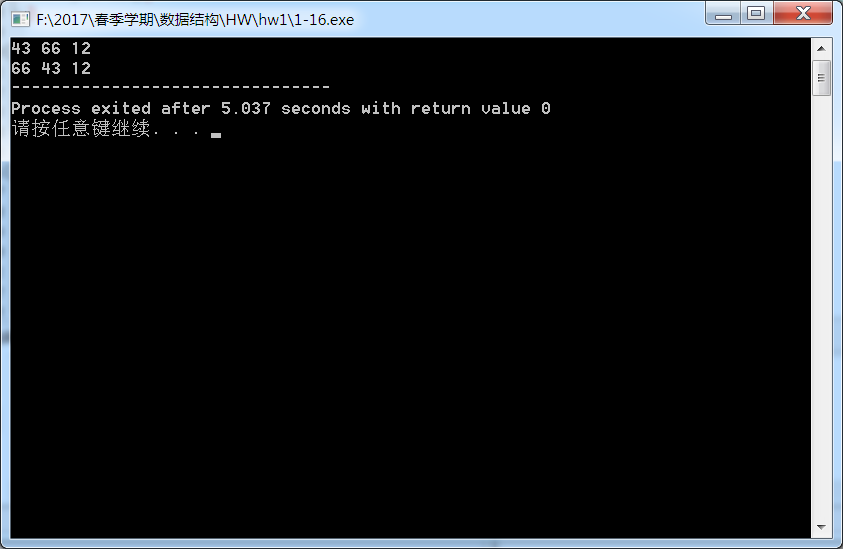
\includegraphics[width=0.75\textwidth]{hw1/screenshot/1-16}
	}
	\item[1.19]
	代码如下.
	\lstinputlisting[language=C]{hw1/1-19.c}
	输入:\fbox{10}
	
	\mbox{
		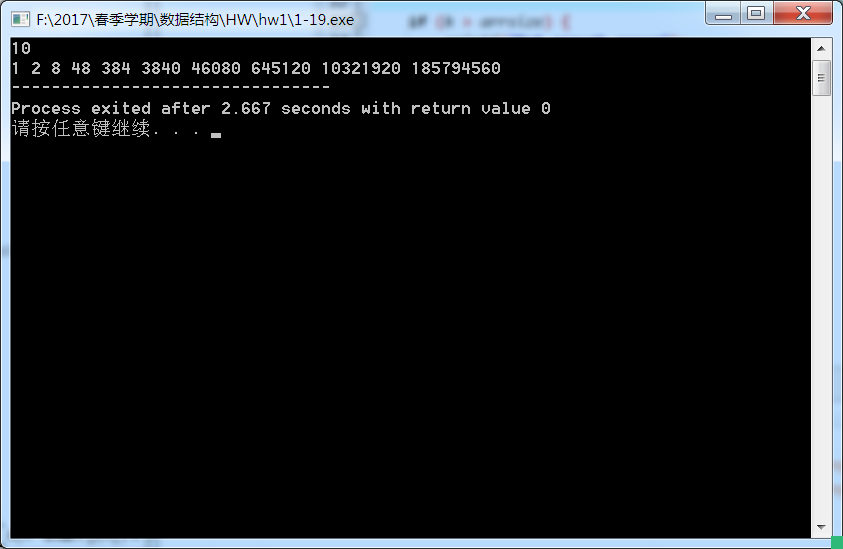
\includegraphics[width=0.75\textwidth]{hw1/screenshot/1-19-success}}
	
	输入:\fbox{200}
	
	\mbox{
		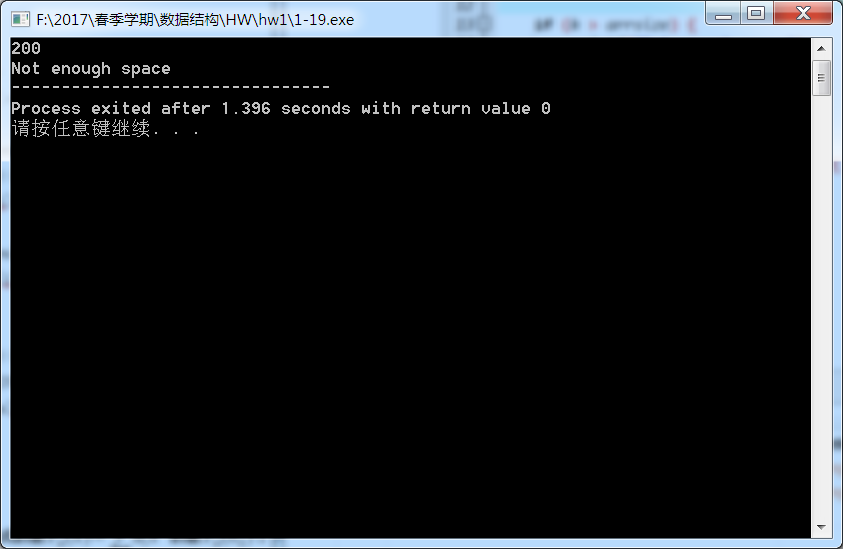
\includegraphics[width=0.75\textwidth]{hw1/screenshot/1-19-space}}
	
	输入:\fbox{15}
	
	\mbox{
		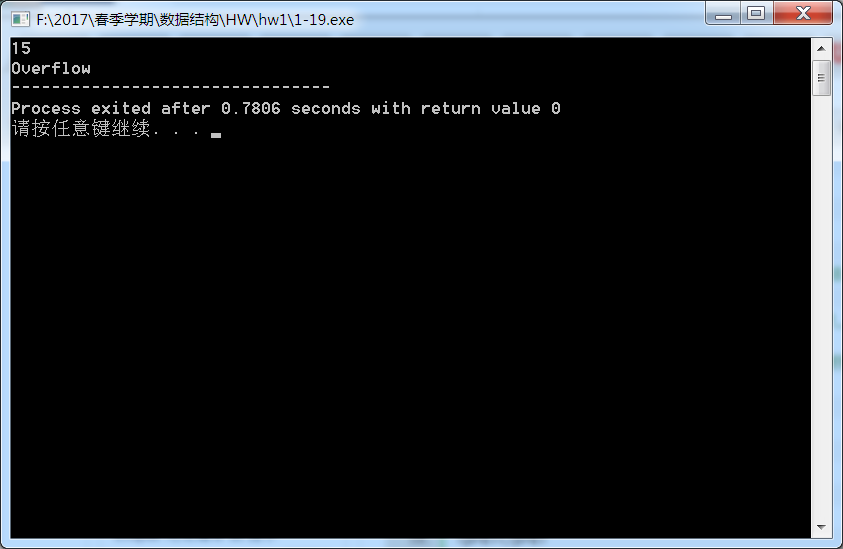
\includegraphics[width=0.75\textwidth]{hw1/screenshot/1-19-overflow}}
	\item[1.20]
	代码如下.
	\lstinputlisting[language=C]{hw1/1-20.c}
	输入函数为$P_1(x)=x+2$,取值$x_0=1.0$:
	
	\mbox{
		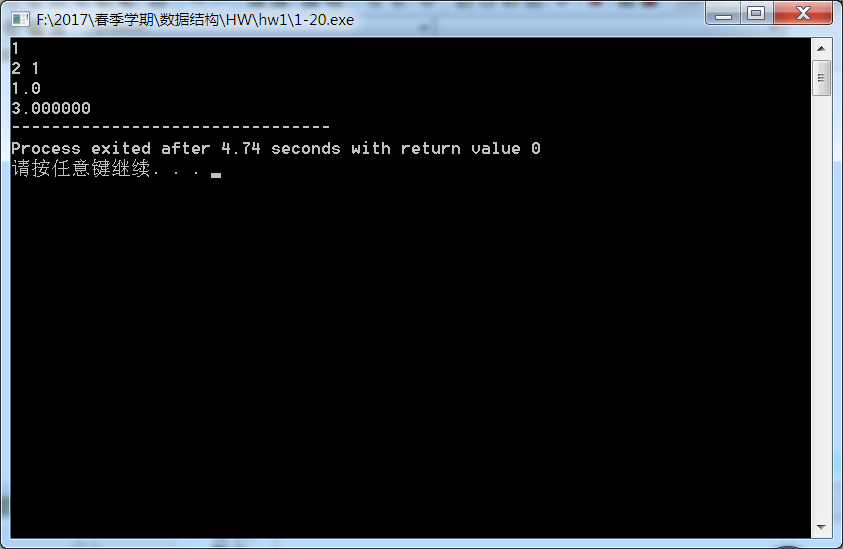
\includegraphics[width=0.75\textwidth]{hw1/screenshot/1-20-linear}}
	
	输入函数为$P_2(x)=x^2+x$,取值$x_0=1.0$:
	
	\mbox{
		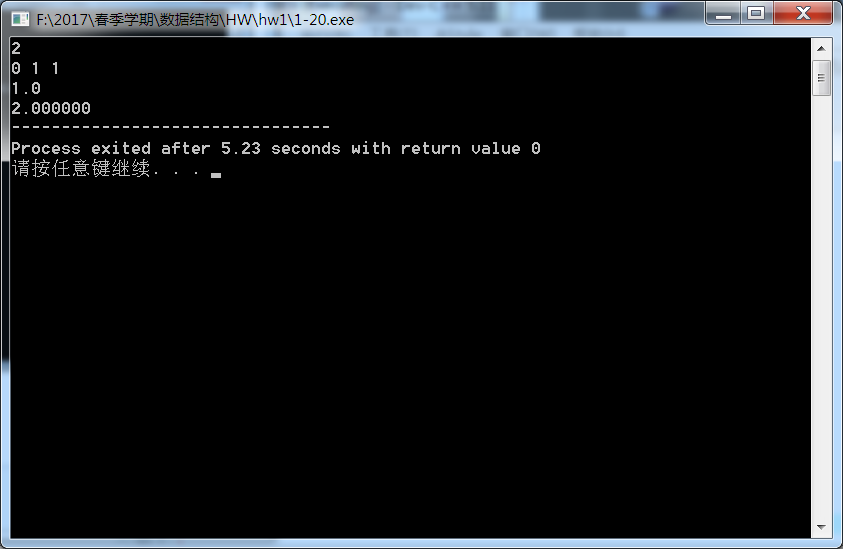
\includegraphics[width=0.75\textwidth]{hw1/screenshot/1-20-quadratic}}
	
	程序中,\texttt{power *= x0;}和\texttt{ans += *(a+i) * power;}的执行频度均为$n$次,整个算法的时间复杂度为$O(n)$.
\end{enumerate}
\newpage
\section*{第2章\ 线性表}
\begin{enumerate}
	\item[2.4]
	示意图如下:
	
	\resizebox{0.95\textwidth}{!}{
		\begin{tabular}{cl}
			(1)&\texttt{Q=P->next;}\\&\begin{tikzpicture}[
	list/.style={
		thick, rectangle split,
		rectangle split parts=2, draw,
		rectangle split horizontal, minimum size=18pt,
		inner sep=4pt, text=black,
		rectangle split part fill={white, blue!20}
	},
	->, start chain, thick
	]
	\node[on chain] (0) {L};
	\node[list,on chain] (1) {2};
	\node[list,on chain] (2) {5};
	\node[list,on chain] (3) {7};
	\node[list,on chain] (4) {3};
	\node[list,on chain] (5) {8};
	\node[on chain] (6) {$\cdots$};
	\node[list,on chain] (7) {6};
	\node[list,on chain] (8) {4\nodepart{two}$\wedge$};
	\foreach \i in {0,...,6}
	{
		\pgfmathsetmacro\next{int(\i + 1)}
		\draw[->] (\i.east) -- (\next .west);
	}
	\draw[*->] let \p1 = (7.two), \p2 = (7.center) in (\x1,\y2) -- (8);
	\node [below = .5cm of 2] (P) {P};
	\draw[->] (P) -- (2);
	\node [below = .5cm of 3] (Q) {Q};
	\draw[->] (Q) -- (3);
	\node [below = .5cm of 4] (R) {R};
	\draw[->] (R) -- (4);
	\node [below = .5cm of 5] (S) {S};
	\draw[->] (S) -- (5);
\end{tikzpicture}\\
			(2)&\texttt{L=P->next;}\\&\begin{tikzpicture}[
	list/.style={
		thick, rectangle split,
		rectangle split parts=2, draw,
		rectangle split horizontal, minimum size=18pt,
		inner sep=4pt, text=black,
		rectangle split part fill={white, blue!20}
	},
	->, start chain, thick
	]
	\node[on chain] (0) {L};
	\node[list,on chain] (3) {7};
	\node[list,on chain] (4) {3};
	\node[list,on chain] (5) {8};
	\node[on chain] (6) {$\cdots$};
	\node[list,on chain] (7) {6};
	\node[list,on chain] (8) {4\nodepart{two}$\wedge$};
	\draw[->] (0.east) -- (3.west);
	\foreach \i in {3,...,6}
	{
		\pgfmathsetmacro\next{int(\i + 1)}
		\draw[->] (\i.east) -- (\next .west);
	}
	\draw[*->] let \p1 = (7.two), \p2 = (7.center) in (\x1,\y2) -- (8);
	\node [below = .5cm of 3] (Q) {Q};
	\draw[->] (Q) -- (3);
	\node [below = .5cm of 4] (R) {R};
	\draw[->] (R) -- (4);
	\node [below = .5cm of 5] (S) {S};
	\draw[->] (S) -- (5);
\end{tikzpicture}\\
			(3)&\texttt{R->data=P->data;}\\&\begin{tikzpicture}[
list/.style={
	thick, rectangle split,
	rectangle split parts=2, draw,
	rectangle split horizontal, minimum size=18pt,
	inner sep=4pt, text=black,
	rectangle split part fill={white, blue!20}
},
->, start chain, thick
]
\node[on chain] (0) {L};
\node[list,on chain] (1) {2};
\node[list,on chain] (2) {5};
\node[list,on chain] (3) {7};
\node[list,on chain] (4) {5};
\node[list,on chain] (5) {8};
\node[on chain] (6) {$\cdots$};
\node[list,on chain] (7) {6};
\node[list,on chain] (8) {4\nodepart{two}$\wedge$};
\foreach \i in {0,...,6}
{
	\pgfmathsetmacro\next{int(\i + 1)}
	\draw[->] (\i.east) -- (\next .west);
}
\draw[*->] let \p1 = (7.two), \p2 = (7.center) in (\x1,\y2) -- (8);
\node [below = .5cm of 2] (P) {P};
\draw[->] (P) -- (2);
\node [below = .5cm of 3] (Q) {Q};
\draw[->] (Q) -- (3);
\node [below = .5cm of 4] (R) {R};
\draw[->] (R) -- (4);
\node [below = .5cm of 5] (S) {S};
\draw[->] (S) -- (5);
\end{tikzpicture}\\
			(4)&\texttt{R->data=P->next->data;}\\&\begin{tikzpicture}[
list/.style={
	thick, rectangle split,
	rectangle split parts=2, draw,
	rectangle split horizontal, minimum size=18pt,
	inner sep=4pt, text=black,
	rectangle split part fill={white, blue!20}
},
->, start chain, thick
]
\node[on chain] (0) {L};
\node[list,on chain] (1) {2};
\node[list,on chain] (2) {5};
\node[list,on chain] (3) {7};
\node[list,on chain] (4) {7};
\node[list,on chain] (5) {8};
\node[on chain] (6) {$\cdots$};
\node[list,on chain] (7) {6};
\node[list,on chain] (8) {4\nodepart{two}$\wedge$};
\foreach \i in {0,...,6}
{
	\pgfmathsetmacro\next{int(\i + 1)}
	\draw[->] (\i.east) -- (\next .west);
}
\draw[*->] let \p1 = (7.two), \p2 = (7.center) in (\x1,\y2) -- (8);
\node [below = .5cm of 2] (P) {P};
\draw[->] (P) -- (2);
\node [below = .5cm of 3] (Q) {Q};
\draw[->] (Q) -- (3);
\node [below = .5cm of 4] (R) {R};
\draw[->] (R) -- (4);
\node [below = .5cm of 5] (S) {S};
\draw[->] (S) -- (5);
\end{tikzpicture}
		\end{tabular}
	}

	\resizebox{0.95\textwidth}{!}{
	\begin{tabular}{cl}
		(5)&\texttt{P->next->next->next->data=P->data;}\\&\begin{tikzpicture}[
list/.style={
	thick, rectangle split,
	rectangle split parts=2, draw,
	rectangle split horizontal, minimum size=18pt,
	inner sep=4pt, text=black,
	rectangle split part fill={white, blue!20}
},
->, start chain, thick
]
\node[on chain] (0) {L};
\node[list,on chain] (1) {2};
\node[list,on chain] (2) {5};
\node[list,on chain] (3) {7};
\node[list,on chain] (4) {3};
\node[list,on chain] (5) {5};
\node[on chain] (6) {$\cdots$};
\node[list,on chain] (7) {6};
\node[list,on chain] (8) {4\nodepart{two}$\wedge$};
\foreach \i in {0,...,6}
{
	\pgfmathsetmacro\next{int(\i + 1)}
	\draw[->] (\i.east) -- (\next .west);
}
\draw[*->] let \p1 = (7.two), \p2 = (7.center) in (\x1,\y2) -- (8);
\node [below = .5cm of 2] (P) {P};
\draw[->] (P) -- (2);
\node [below = .5cm of 3] (Q) {Q};
\draw[->] (Q) -- (3);
\node [below = .5cm of 4] (R) {R};
\draw[->] (R) -- (4);
\node [below = .5cm of 5] (S) {S};
\draw[->] (S) -- (5);
\end{tikzpicture}\\
		(6)&\texttt{T=P; \textbf{while} (T!=NULL)\{T->data=T->data*2;T=T->next;\}}\\&\begin{tikzpicture}[
list/.style={
	thick, rectangle split,
	rectangle split parts=2, draw,
	rectangle split horizontal, minimum size=18pt,
	inner sep=4pt, text=black,
	rectangle split part fill={white, blue!20}
},
->, start chain, thick
]
\node[on chain] (0) {L};
\node[list,on chain] (1) {2};
\node[list,on chain] (2) {10};
\node[list,on chain] (3) {14};
\node[list,on chain] (4) {6};
\node[list,on chain] (5) {16};
\node[on chain] (6) {$\cdots$};
\node[list,on chain] (7) {12};
\node[list,on chain] (8) {8\nodepart{two}$\wedge$};
\foreach \i in {0,...,6}
{
	\pgfmathsetmacro\next{int(\i + 1)}
	\draw[->] (\i.east) -- (\next .west);
}
\draw[*->] let \p1 = (7.two), \p2 = (7.center) in (\x1,\y2) -- (8);
\node [below = .5cm of 2] (P) {P};
\draw[->] (P) -- (2);
\node [below = .5cm of 3] (Q) {Q};
\draw[->] (Q) -- (3);
\node [below = .5cm of 4] (R) {R};
\draw[->] (R) -- (4);
\node [below = .5cm of 5] (S) {S};
\draw[->] (S) -- (5);
\end{tikzpicture}\\
		(7)&\texttt{T=P; \textbf{while} (T->next!=NULL)\{T->data=T->data*2;T=T->next;\}}\\&\begin{tikzpicture}[
list/.style={
	thick, rectangle split,
	rectangle split parts=2, draw,
	rectangle split horizontal, minimum size=18pt,
	inner sep=4pt, text=black,
	rectangle split part fill={white, blue!20}
},
->, start chain, thick
]
\node[on chain] (0) {L};
\node[list,on chain] (1) {2};
\node[list,on chain] (2) {10};
\node[list,on chain] (3) {14};
\node[list,on chain] (4) {6};
\node[list,on chain] (5) {16};
\node[on chain] (6) {$\cdots$};
\node[list,on chain] (7) {12};
\node[list,on chain] (8) {4\nodepart{two}$\wedge$};
\foreach \i in {0,...,6}
{
	\pgfmathsetmacro\next{int(\i + 1)}
	\draw[->] (\i.east) -- (\next .west);
}
\draw[*->] let \p1 = (7.two), \p2 = (7.center) in (\x1,\y2) -- (8);
\node [below = .5cm of 2] (P) {P};
\draw[->] (P) -- (2);
\node [below = .5cm of 3] (Q) {Q};
\draw[->] (Q) -- (3);
\node [below = .5cm of 4] (R) {R};
\draw[->] (R) -- (4);
\node [below = .5cm of 5] (S) {S};
\draw[->] (S) -- (5);
\end{tikzpicture}
	\end{tabular}
}
	\item[2.5]
	示意图如下:
	
	\resizebox{0.95\textwidth}{!}{
		\begin{tabular}{l}
			\texttt{L=(LinkList)\textbf{malloc}(\textbf{sizeof}(LNode)); P=L;}\\\begin{tikzpicture}[
list/.style={
	thick, rectangle split,
	rectangle split parts=2, draw,
	rectangle split horizontal, minimum size=18pt,
	inner sep=4pt, text=black,
	rectangle split part fill={white, blue!20}
},
->, start chain, thick
]
\node[on chain] (0) {L};
\node[list,on chain] (1) {};
\draw[->] (0.east) -- (1.west);
\node [below = .5cm of 1] (P) {P};
\draw[->] (P) -- (1);
\end{tikzpicture}\\
			\texttt{\textbf{for} (i=1;i<=4;i++)\{P->next=(LinkList)\textbf{malloc}(\textbf{sizeof}(LNode)); P=P->next; P->data=i*2-1;}\}\\\begin{tikzpicture}[
list/.style={
	thick, rectangle split,
	rectangle split parts=2, draw,
	rectangle split horizontal, minimum size=18pt,
	inner sep=4pt, text=black,
	rectangle split part fill={white, blue!20}
},
->, start chain, thick
]
\node[on chain] (0) {L};
\node[list,on chain] (1) {};
\node[list,on chain] (2) {1};
\node[list,on chain] (3) {3};
\node[list,on chain] (4) {5};
\node[list,on chain] (5) {7};
\foreach \i in {0,...,4}
{
	\pgfmathsetmacro\next{int(\i + 1)}
	\draw[->] (\i.east) -- (\next .west);
}
\node [below = .5cm of 5] (P) {P};
\draw[->] (P) -- (5);
\end{tikzpicture}\\
			\texttt{P->next=\textbf{NULL};}\\\begin{tikzpicture}[
list/.style={
	thick, rectangle split,
	rectangle split parts=2, draw,
	rectangle split horizontal, minimum size=18pt,
	inner sep=4pt, text=black,
	rectangle split part fill={white, blue!20}
},
->, start chain, thick
]
\node[on chain] (0) {L};
\node[list,on chain] (1) {};
\node[list,on chain] (2) {1};
\node[list,on chain] (3) {3};
\node[list,on chain] (4) {5};
\node[list,on chain] (5) {7\nodepart{two}$\wedge$};
\foreach \i in {0,...,3}
{
	\pgfmathsetmacro\next{int(\i + 1)}
	\draw[->] (\i.east) -- (\next .west);
}
\draw[*->] let \p1 = (4.two), \p2 = (4.center) in (\x1,\y2) -- (5);
\node [below = .5cm of 5] (P) {P};
\draw[->] (P) -- (5);
\end{tikzpicture}
		\end{tabular}
	}

	\resizebox{0.95\textwidth}{!}{
		\begin{tabular}{l}
			\texttt{\textbf{for} (i=4;i>=1;i--) Ins\_LinkList(L,i+1,i*2);}\\\begin{tikzpicture}[
list/.style={
	thick, rectangle split,
	rectangle split parts=2, draw,
	rectangle split horizontal, minimum size=18pt,
	inner sep=4pt, text=black,
	rectangle split part fill={white, blue!20}
},
->, start chain, thick
]
\node[on chain] (0) {L};
\node[list,on chain] (1) {};
\node[list,on chain] (2) {1};
\node[list,on chain] (3) {2};
\node[list,on chain] (4) {3};
\node[list,on chain] (5) {4};
\node[list,on chain] (6) {5};
\node[list,on chain] (7) {6};
\node[list,on chain] (8) {7};
\node[list,on chain] (9) {8\nodepart{two}$\wedge$};
\foreach \i in {0,...,7}
{
	\pgfmathsetmacro\next{int(\i + 1)}
	\draw[->] (\i.east) -- (\next .west);
}
\draw[*->] let \p1 = (8.two), \p2 = (8.center) in (\x1,\y2) -- (9);
\node [below = .5cm of 9] (P) {P};
\draw[->] (P) -- (9);
\end{tikzpicture}\\
			\texttt{\textbf{for} (i=1;i<=3;i++) Del\_LinkList(L,i);}\\\begin{tikzpicture}[
list/.style={
	thick, rectangle split,
	rectangle split parts=2, draw,
	rectangle split horizontal, minimum size=18pt,
	inner sep=4pt, text=black,
	rectangle split part fill={white, blue!20}
},
->, start chain, thick
]
\node[on chain] (0) {L};
\node[list,on chain] (1) {};
\node[list,on chain] (2) {2};
\node[list,on chain] (3) {4};
\node[list,on chain] (4) {6};
\node[list,on chain] (5) {7};
\node[list,on chain] (6) {8\nodepart{two}$\wedge$};
\foreach \i in {0,...,4}
{
	\pgfmathsetmacro\next{int(\i + 1)}
	\draw[->] (\i.east) -- (\next .west);
}
\draw[*->] let \p1 = (5.two), \p2 = (5.center) in (\x1,\y2) -- (6);
\node [below = .5cm of 6] (P) {P};
\draw[->] (P) -- (6);
\end{tikzpicture}
		\end{tabular}
	}
	\item[2.9](1) 若表\texttt{L}的长度不小于$2$,将\texttt{L}的首结点变成尾结点;
	
	(2) BB把单循环链表中的两个结点直接连接起来,AA利用BB将一个单循环链表拆成两个单循环链表.
	%
	\item[2.11]
	代码如下.
	\lstinputlisting[language=C]{hw1/2-11.c}
	向有序表\texttt{va = \{1, 2, 3, 5, 6, 7, 8\}}中依次插入元素$4$、$9$、$0$和$-5$(检查在中间和两边插入):
	
	\mbox{
		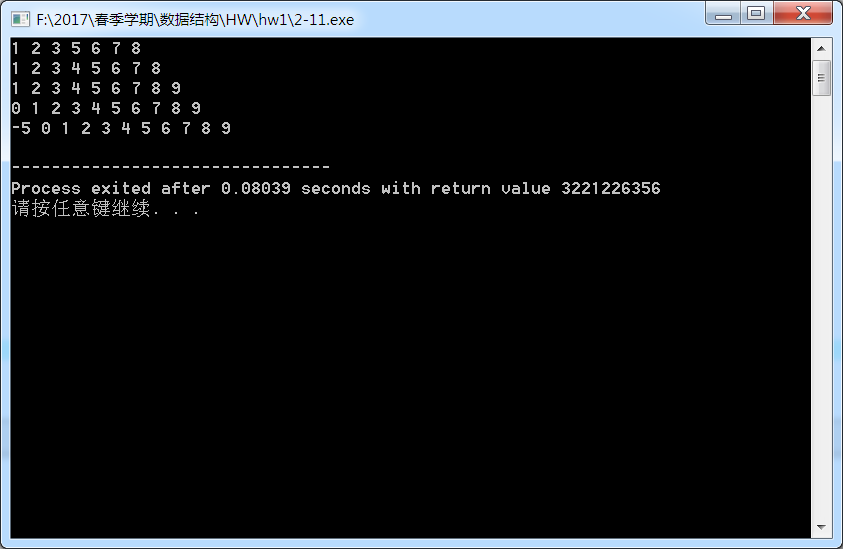
\includegraphics[width=0.75\textwidth]{hw1/screenshot/2-11}}
	\item[2.12]
	代码如下.
	\lstinputlisting[language=C]{hw1/2-12.c}
	创建四个线性表\texttt{L = \{1, 2, 3, 4, 5, 6, 7\}, M = \{1, 2, 3, 5, 6, 7, 8\}, N = O = \{1, 2, 3, 5, 6, 7, 8, 9\}},比较结果如下:
	
	\mbox{
		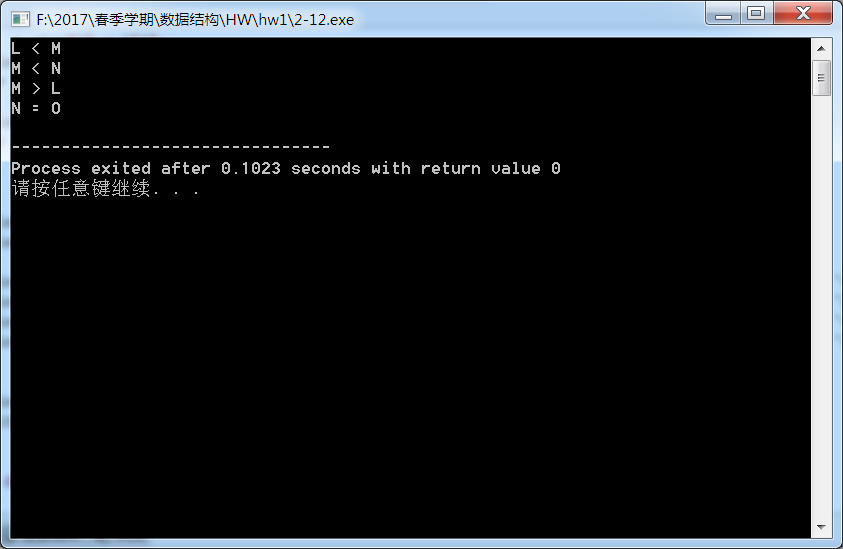
\includegraphics[width=0.75\textwidth]{hw1/screenshot/2-12}}
	\item[2.19]
	代码如下.
	\lstinputlisting[language=C]{hw1/2-19.c}
	创建单链表\texttt{L = \{1, 2, 3, 5, 6, 7, 8, 9, 10\}},输入\texttt{mink}=\fbox{3},\texttt{maxk}=\fbox{7}:
	
	\mbox{
		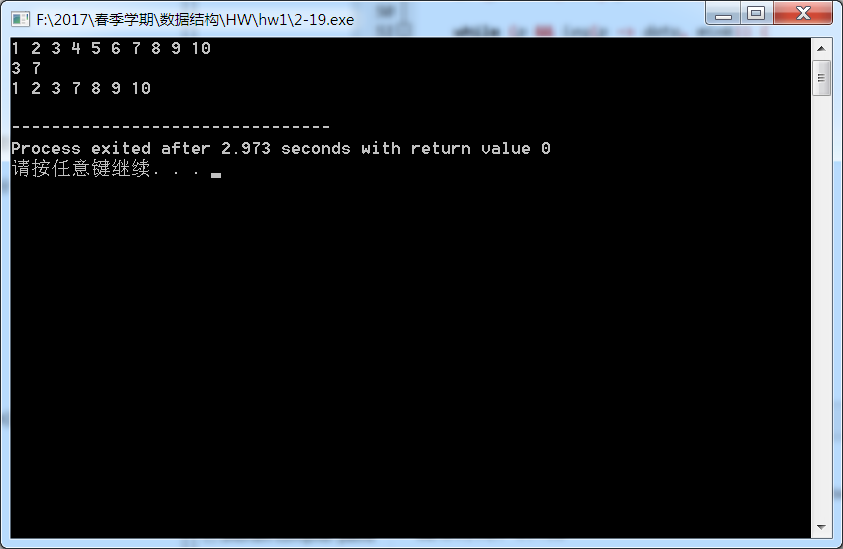
\includegraphics[width=0.75\textwidth]{hw1/screenshot/2-19}}
	
	时间复杂度为$O(\mathtt{maxk})$.
	\item[2.22]
	代码如下.
	\lstinputlisting[language=C]{hw1/2-22.c}
	
	原地逆置单链表\texttt{L = \{1, 2, 3, 5, 6, 7, 8, 9, 10\}}:
	
	\mbox{
		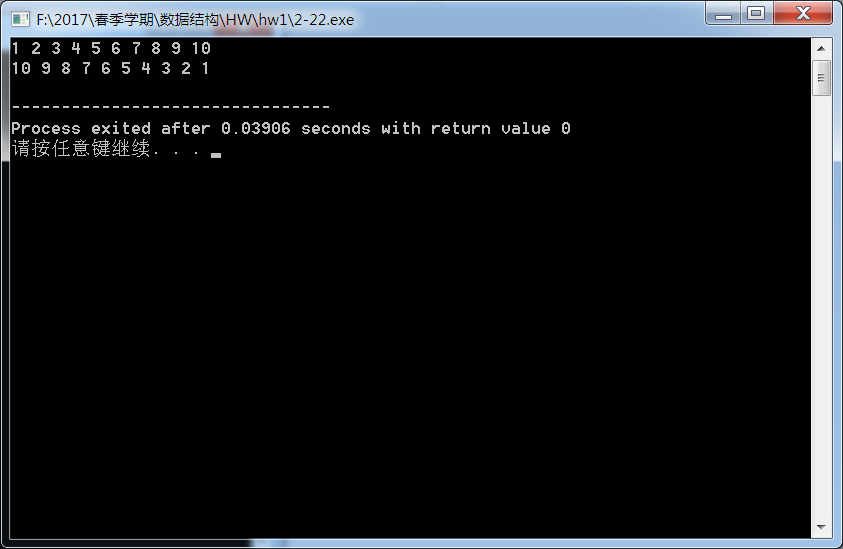
\includegraphics[width=0.75\textwidth]{hw1/screenshot/2-22}}
	\item[2.29]
	代码如下.
	\lstinputlisting[language=C]{hw1/2-29.c}
	
	从表\texttt{A = \{1, 2, 3, 4, 5, 6, 7, 7\}}中删除表\texttt{B = \{0, 2, 3, 4, 6, 7, 9, 9\}}和\texttt{C = \{1, 2, 3, 6, 7, 8, 9, 9\}}的共同元素:
	
	\mbox{
		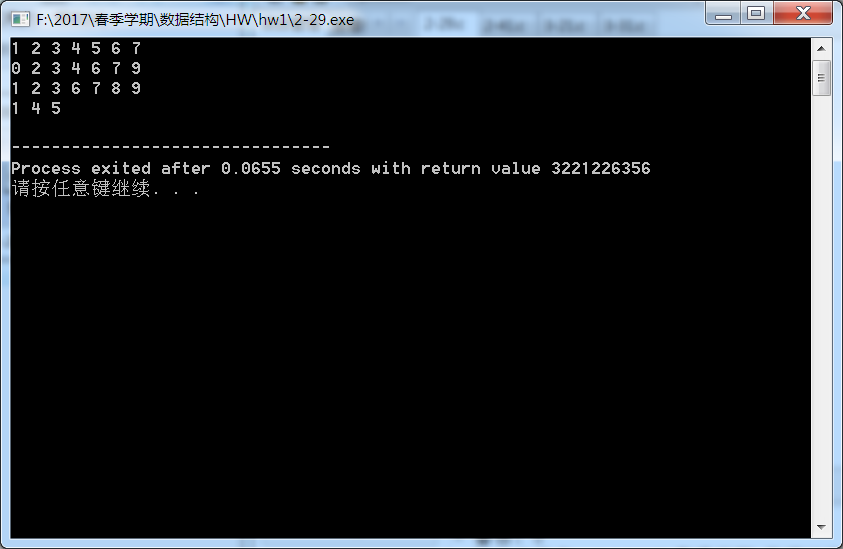
\includegraphics[width=0.75\textwidth]{hw1/screenshot/2-29}}
	\item[2.41]
	代码如下.
	\lstinputlisting[language=C]{hw1/2-41.c}
	
	首先读入多项式的最高项次数$n=$\fbox{$3$},然后次数由低到高依次读入各项系数\fbox{$1,1,1,2$},对多项式$2x^3+x^2+x+1$求导:
	
	\mbox{
		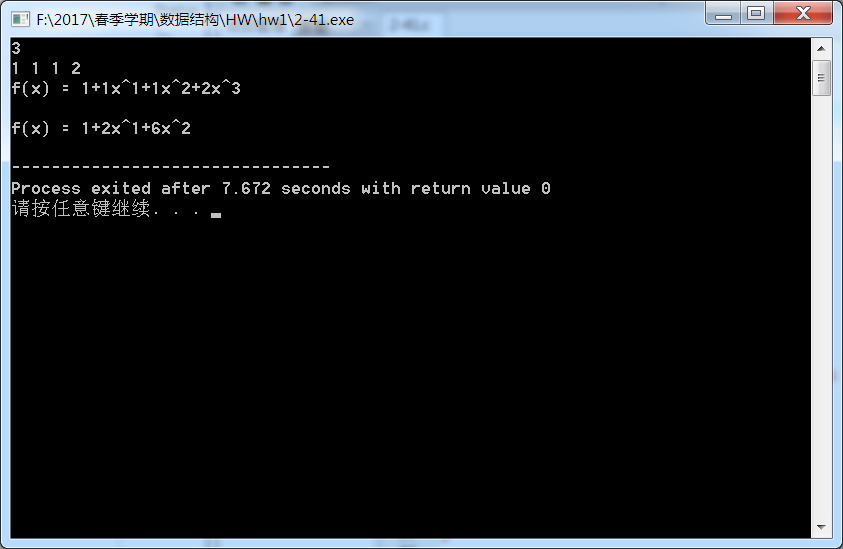
\includegraphics[width=0.75\textwidth]{hw1/screenshot/2-41}}
\end{enumerate}
\end{document}